\documentclass[11pt,a4paper]{article}
\usepackage{fontspec}
\setmainfont{TeX Gyre Pagella}
\newfontfamily\headfont{Inter}[UprightFont=*-ExtraBold,BoldFont=*-ExtraBold,Extension=.otf,Path=/usr/share/fonts/opentype/inter/]
\usepackage[a4paper,margin=2.3cm]{geometry}
\usepackage{graphicx,booktabs,float,caption,array,xcolor,longtable}
\usepackage{xurl}
\usepackage[hidelinks]{hyperref}
\usepackage{titlesec}
\usepackage[round]{natbib}
\usepackage{setspace}
\setstretch{1.05}
\renewcommand{\topfraction}{0.9}
\renewcommand{\bottomfraction}{0.8}
\renewcommand{\textfraction}{0.1}
\renewcommand{\floatpagefraction}{0.75}
\setlength{\parindent}{0pt}
\setlength{\parskip}{0.55em}
\titleformat{\section}{\headfont\Large}{\thesection}{0.8em}{}
\titleformat{\subsection}{\headfont\large}{\thesubsection}{0.8em}{}
\captionsetup{font=small,labelfont=bf}
\urlstyle{same}
\hypersetup{pdftitle={Who's on the Moon?},pdfauthor={Tristan Hotham}}

\begin{document}
\begin{center}
{\Large\bfseries Who's on the Moon?\par}
\vspace{0.4em}
{\large The birthplaces of the people that features on the Moon,\\Mercury, Venus and Mars are named after\par}
\vspace{1.2em}
{\large Tristan Hotham\par}
\vspace{0.3em}
{\small Independent researcher\\
ORCID: 0000-0003-4931-9349\\
DOI: https://doi.org/10.5281/zenodo.24055578\par}
\vspace{0.8em}
2026
\end{center}

\begin{quote}
\small
\begin{center}\textbf{Abstract}\end{center}
Thousands of surface features on the Moon, Mercury, Venus and Mars are named after people. Using Wikidata's "named after" statements, I link 3,471 named features on the four bodies to the 2,560 people that 2,718 of them honour, and those people to their birthplaces on Earth. Of the lunar features named after a person with a known birthplace, 75.3\% honour someone born in Europe, against 54.9\% on Mercury, 61.5\% on Venus and 64.8\% on Mars. Paris is the birthplace of 38 lunar namesakes, more than Africa, South America and Oceania together (31). The naming rules of each body show clearly: 52.0\% of the Moon's namesakes were astronomers, while 97.6\% of Mercury's had an artistic or literary occupation. On the lunar far side, named after the Soviet Luna 3 images of 1959, 19.9\% of namesakes were born in the former Soviet Union, against 3.5\% on the near side, and the median namesake was born in 1874 rather than 1784. Women are 2.8\% of the Moon's namesakes, 17.8\% of Mercury's and 5.5\% of Mars's (Venus honours women by rule), rising to 30.9\% of namesakes born since 1940. The 279 Martian features named after places on Earth, mostly small craters named after villages, come from 102 countries and are far less European (30.4\%) than Mars's people. I describe the data, its gaps and the errors it contains, and publish the linked tables and an interactive map.

\textbf{Keywords:} planetary nomenclature; Moon; Mercury; Venus; Mars; toponymy; commemoration; Eurocentrism; Wikidata; open data; mapping
\end{quote}

\section{Introduction}
The names on the Moon are a record of who was thought worth remembering, and by whom. The near side's craters were largely named in the seventeenth century, when Giovanni Battista Riccioli's \textit{Almagestum Novum} \citep{riccioli} set out the scheme of honouring astronomers and philosophers that has lasted ever since \citep{whitaker}. Today the International Astronomical Union (IAU), founded in 1919, standardises the names of features on other bodies, and its Working Group for Planetary System Nomenclature keeps the official Gazetteer \citep{gazetteer}. Each body has its own themes: lunar craters honour deceased scientists, scholars and explorers; Mercury's craters honour deceased artists, musicians, painters and authors; features on Venus are named after women, real and mythological; large Martian craters honour deceased scientists and writers connected with Mars, and small ones are named after villages on Earth \citep{gazetteer}.

These rules say what kind of person is honoured, not where they came from. This paper asks that second question with open data. Wikidata \citep{wikidata} records, for many planetary features, what they are named after (property P138) and, for many people, where they were born (P19). Joining the two gives each named feature a place on Earth. The result is a map of the geography of commemoration beyond Earth: whose countries, centuries and occupations the other worlds remember.

\section{Data}
The data come from a single query of Wikidata through the QLever SPARQL engine \citep{qlever}: every item with coordinates on the Moon (Q405), Mars (Q111), Mercury (Q308) or Venus (Q313) that has a "named after" statement, with the type of feature, its diameter, the namesake and, where the namesake is a person (Q5), their place of birth, its coordinates and country, dates of birth and death, occupations and number of Wikipedia sitelinks. The query returned 19,194 rows, one for every combination of feature type and occupation. Wikidata is released under CC0.

After deduplication (Section~\ref{sec:methods}) there are 3,471 features: 1,847 on the Moon, 522 on Mercury, 518 on Venus and 584 on Mars. 90 map quadrangles, which take the name of a feature on them, are excluded. 2,718 feature and person pairs (``namings'') involve 2,560 distinct people, of whom 2,416 have a birthplace with coordinates. Table~\ref{tab:bodies} summarises the four bodies.

\begin{table}[tbp]\centering\small\caption{The four bodies. Namings: feature and person pairs; located: with a birthplace with coordinates.}\label{tab:bodies}\begin{tabular}{lrrrr}\toprule & Moon & Mercury & Venus & Mars\\\midrule
Named features & 1,847 & 522 & 518 & 584\\
Named after a person (\%) & 85.7 & 86.8 & 79.3 & 40.1\\
Namings & 1,614 & 457 & 412 & 235\\
Located namings & 1,548 & 426 & 384 & 216\\
Born in Europe (\%) & 75.3 & 54.9 & 61.5 & 64.8\\
Modern countries & 73 & 77 & 52 & 32\\
Median year of birth & 1838 & 1820 & 1852 & 1862\\
Top country & U. States & U. States & U. States & U. States\\
\bottomrule\end{tabular}\end{table}

Natural Earth's 1:10m countries \citep{naturalearth} give each birthplace a modern country and continent.

\section{Methods}\label{sec:methods}
\subsection{Deduplication and linking}
Rows were reduced to one per feature and namesake. 40 features are named after more than one person (for example a crater shared by two astronomers of the same name) and contribute one naming for each. A person with more than one birthplace in Wikidata (52 people) keeps the first that has coordinates. Feature longitudes were converted to $-180$ to $180$ degrees, east positive. Feature types were grouped into craters, crater chains, mountains, valleys and rilles, plains and seas, and scarps and ridges. One namesake label vandalised in Wikidata was corrected, missing labels were supplied, and a few birthplaces, sex values and place links were corrected in documented overrides files (Section~\ref{sec:errors}). Sex comes from a second query (property P21); shares of women are among namesakes recorded as female or male. Places on Earth that features are named after come from a third query, keeping namesakes with coordinates on Earth and excluding languages.

\subsection{Country, continent and the former Soviet Union}
Each birthplace was placed in a Natural Earth country polygon by its coordinates; 144 people without coordinates are excluded from geographic shares. Countries are modern: Ptolemy, born in Ptolemais Hermiou, counts for Egypt, and David Hilbert, born in K\"onigsberg, for Russia. ``Former Soviet Union'' means the fifteen countries that were Soviet republics. Shares are of namings with a located birthplace; a person honoured on two bodies counts on each.

\subsection{Occupations}
Wikidata occupations were mapped to seven groups by keyword, in priority order: astronauts and cosmonauts; astronomers; other scientists, mathematicians and engineers; writers, artists and musicians; explorers, navigators and aviators; philosophers, scholars and religious figures; and rulers, politicians and others. Each person is placed in the first group any of their occupations matches; shares leave out the few people with no occupation recorded. Because many people had several occupations, I also report the share with at least one artistic or literary occupation.

\subsection{Near and far side}
A lunar feature is on the far side if its longitude is more than 90 degrees east or west, the conventional boundary; libration lets observers on Earth see a little beyond it.

\section{Results}
\subsection{Continents}
Figure~\ref{fig:world} maps every located birthplace. On the Moon, 1,165 of 1,548 located namings (75.3\%) are of people born in Europe, 250 (16.1\%) in North America and 102 (6.6\%) in Asia, 58 of whom were born before 1500 (Turkey, the birthplace of many Ionian Greek scholars, has 32). Africa has 19, 12 of them in Egypt; South America 6; Oceania 6. The single city of Paris (38) outnumbers those three continents. The other bodies are less European (Figure~\ref{fig:cont}): Mercury, named after artists from every tradition, has 54.9\% European and 19.7\% Asian namesakes; Venus 61.5\% and Mars 64.8\% European. Over all four, 69.0\% of located namings are European, from 104 modern countries.

\begin{figure}[tbp]\centering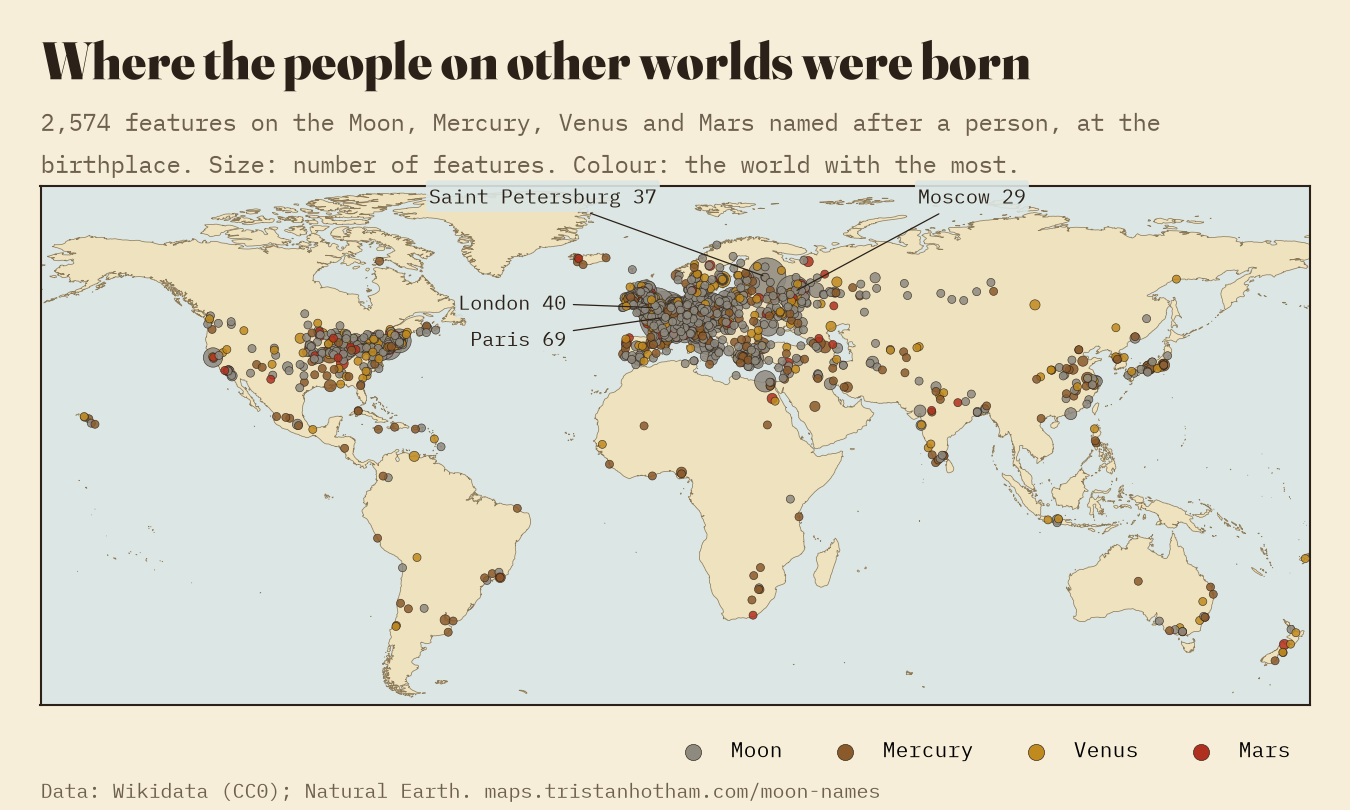
\includegraphics[width=\textwidth]{f_world.png}
\caption{Birthplaces of the people that features on the four bodies are named after. Circle area: number of features; colour: the body with most.}\label{fig:world}\end{figure}
\begin{figure}[tbp]\centering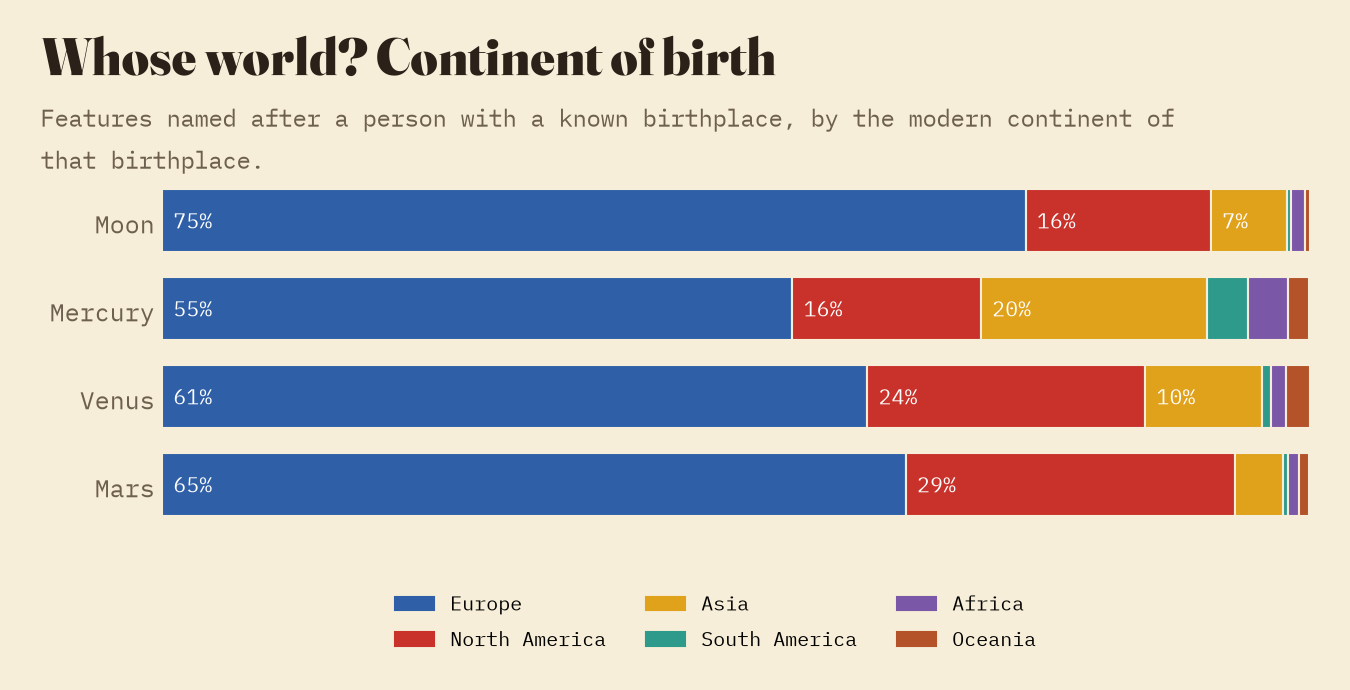
\includegraphics[width=\textwidth]{f_continents.png}
\caption{Continent of birth of namesakes, by body.}\label{fig:cont}\end{figure}

\subsection{Countries}
Four countries dominate the Moon: the United States (15.1\%), Germany (13.1\%), the United Kingdom (12.4\%) and France (10.8\%); Germany, France and Britain together account for 36.3\% (Figure~\ref{fig:cty}). China has 15 lunar namings, India 10 and Japan 9. The United States leads more strongly on Venus (23.2\%) and Mars (28.2\%), where many features were named in the space age after American scientists and, on Venus, American women.

\begin{figure}[tbp]\centering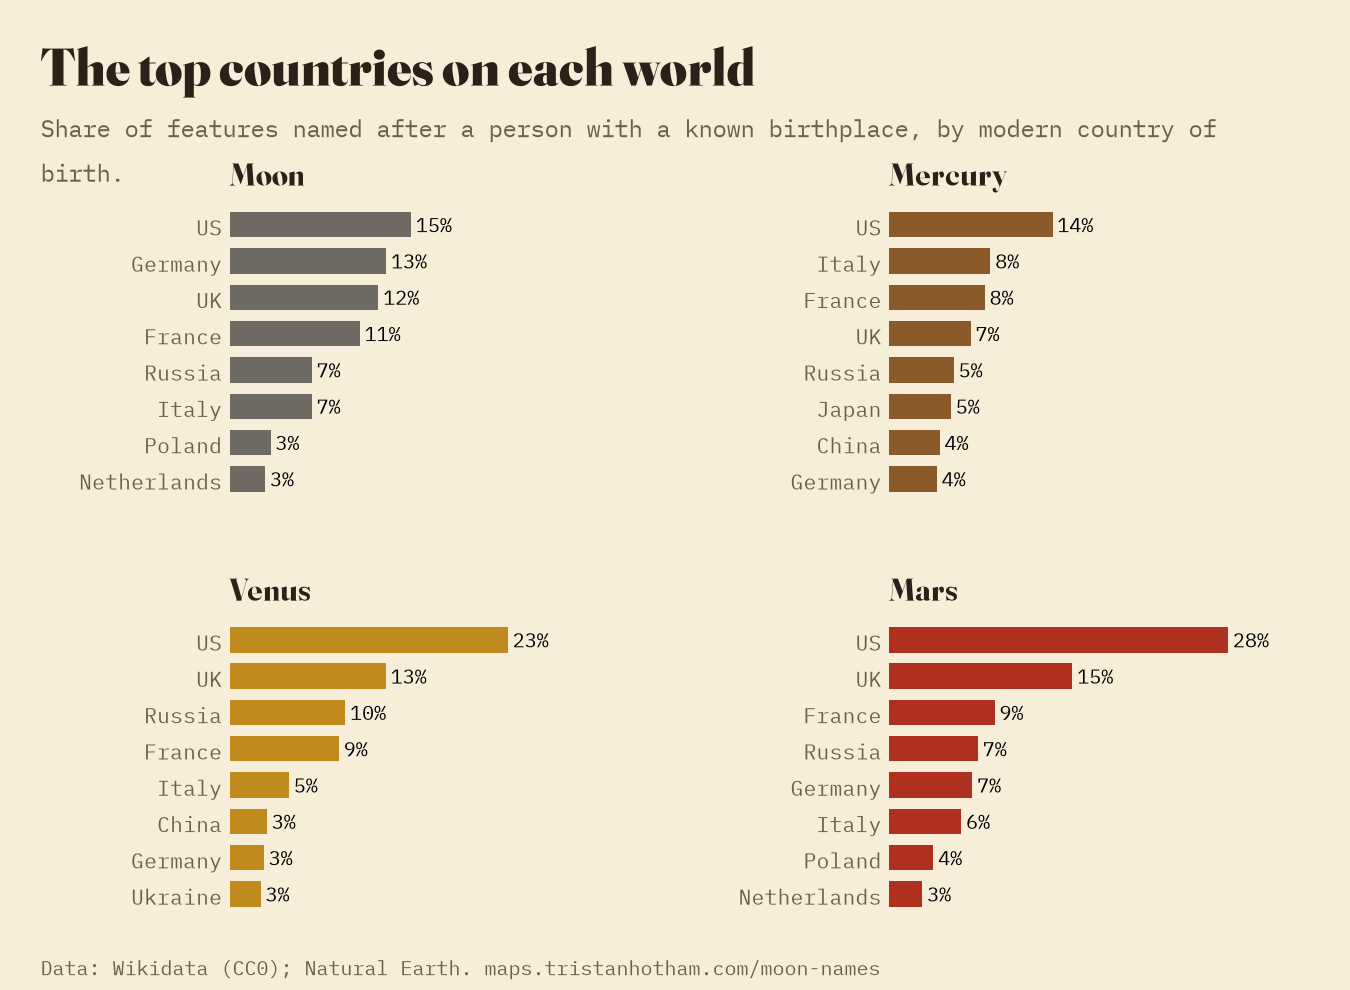
\includegraphics[width=\textwidth]{f_countries.png}
\caption{The eight most common modern countries of birth on each body.}\label{fig:cty}\end{figure}

\subsection{Centuries and occupations}
The Moon's median namesake was born in 1838, Mercury's in 1820, Venus's in 1852 and Mars's in 1862 (Figure~\ref{fig:cent}). The Moon holds the oldest names (178 of its namings honour people born before 1500) but its largest cohort was born in the nineteenth century. Occupations follow the IAU's rules closely (Figure~\ref{fig:occ}): 52.0\% of lunar namesakes were astronomers and 40.2\% other scientists; on Mercury 89.7\% fall first in the arts group and 97.6\% have at least one artistic or literary occupation; Venus, with its rule for women, has the largest share of rulers, politicians and others (10.1\%).

\begin{figure}[tbp]\centering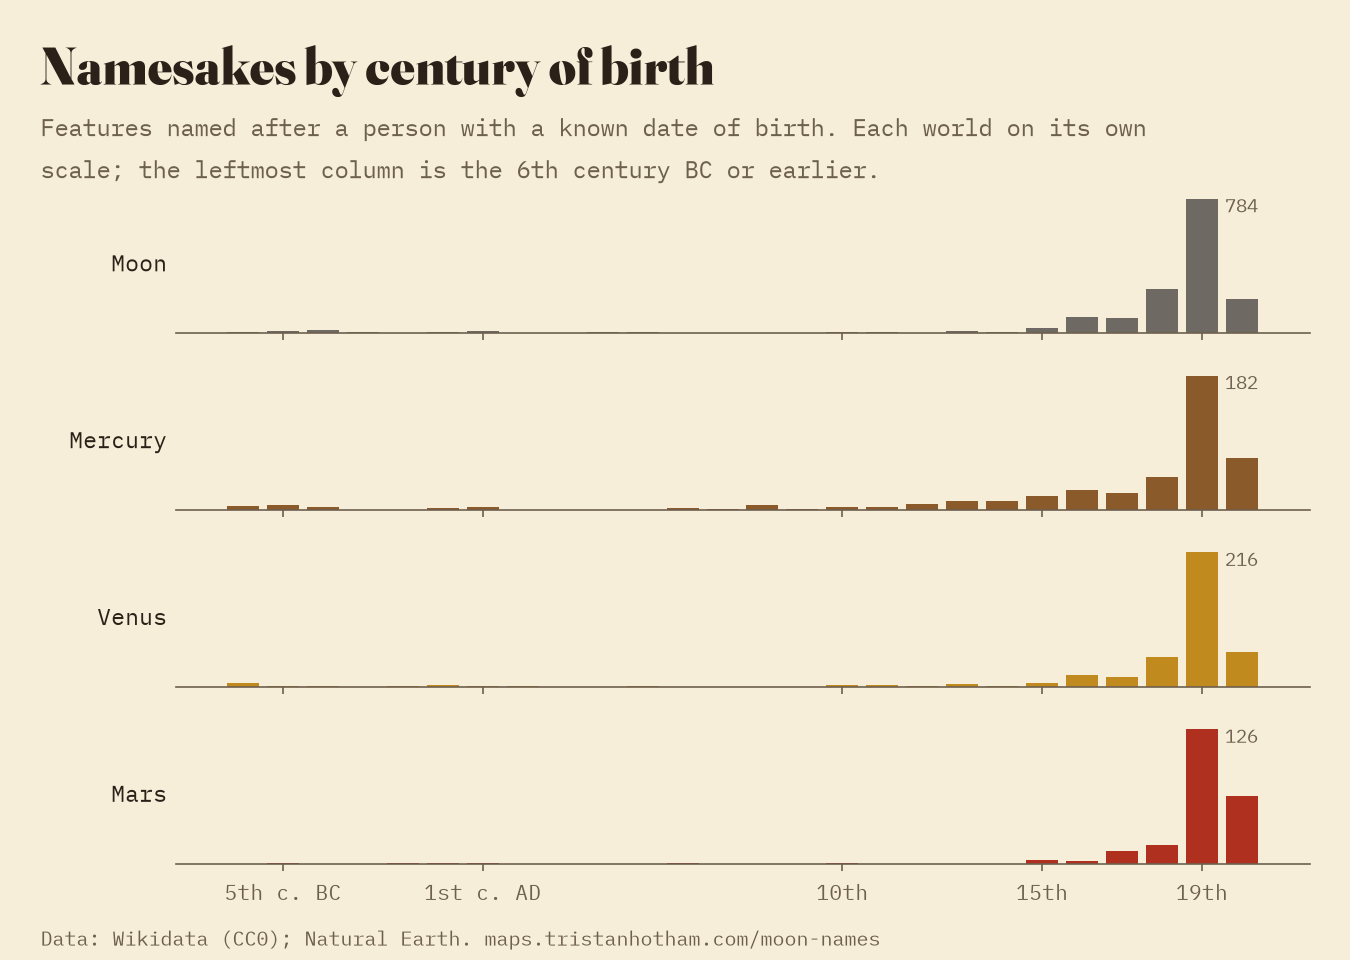
\includegraphics[width=\textwidth]{f_centuries.png}
\caption{Namesakes by century of birth. Each body is on its own scale.}\label{fig:cent}\end{figure}
\begin{figure}[tbp]\centering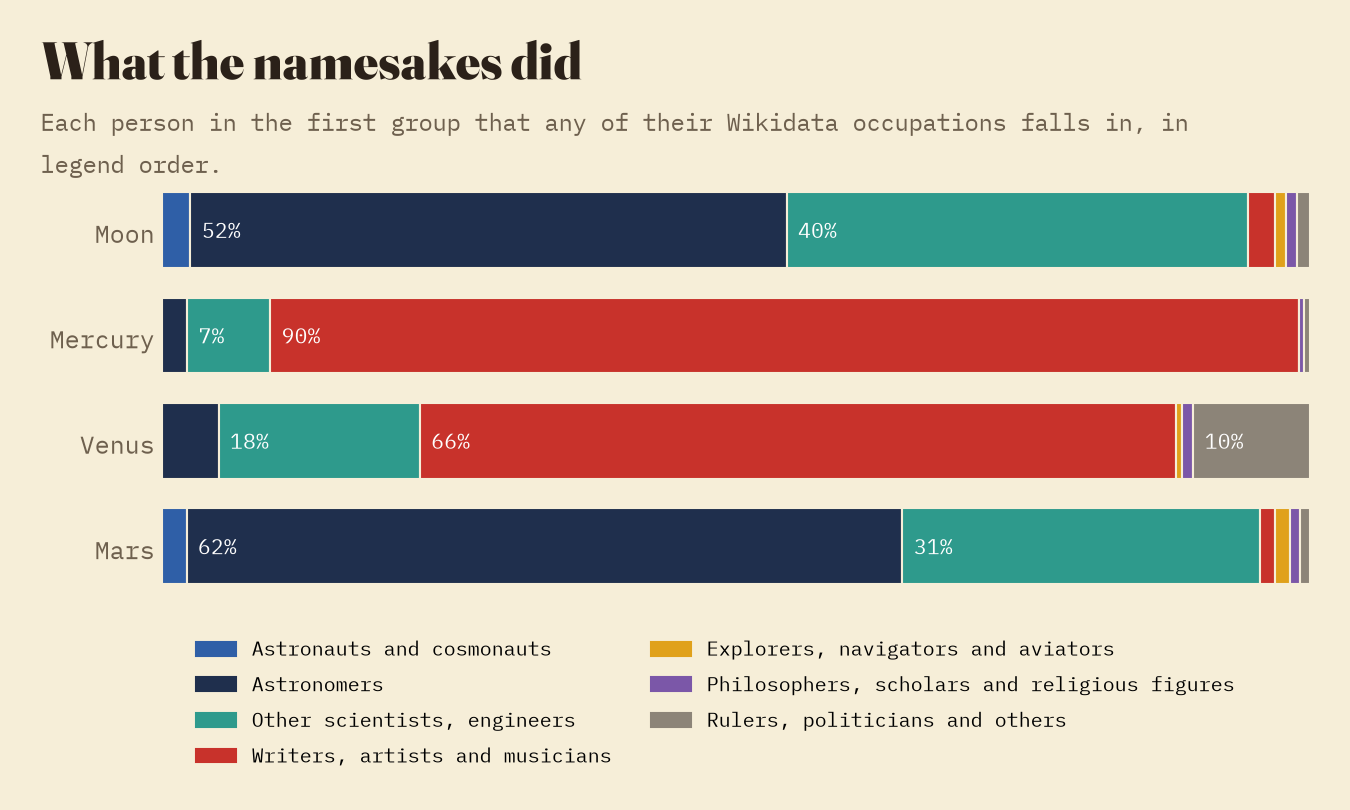
\includegraphics[width=\textwidth]{f_occupations.png}
\caption{Occupation groups of namesakes by body.}\label{fig:occ}\end{figure}

\subsection{The far side}
The far side of the Moon was first photographed by the Soviet probe Luna 3 in 1959, and most of its features were named in the following decades, many after Soviet proposals \citep{whitaker}. The birthplaces show it (Table~\ref{tab:far}, Figure~\ref{fig:faces}): 19.9\% of far-side namings are of people born in the former Soviet Union, 5.7 times the near side's 3.5\%. Far-side namesakes are also younger and more often American, and include 35 astronauts and cosmonauts, among them Yuri Gagarin, Valentina Tereshkova and the crews of Apollo 1, Challenger and Columbia.

\begin{table}[tbp]\centering\small\caption{Near side and far side of the Moon.}\label{tab:far}\begin{tabular}{lrr}\toprule & Near side & Far side\\\midrule
Namings & 934 & 678\\
Located & 889 & 657\\
Born in former USSR (\%) & 3.5 & 19.9\\
Born in Russia & 21 & 85\\
Born in Europe (\%) & 79.0 & 70.2\\
Born in the United States (\%) & 11.5 & 20.1\\
Median year of birth & 1784 & 1874\\
Astronomers (\%) & 58.9 & 42.3\\
Other scientists (\%) & 33.3 & 49.4\\
Astronauts and cosmonauts & 4 & 36\\
\bottomrule\end{tabular}\end{table}

\begin{figure}[tbp]\centering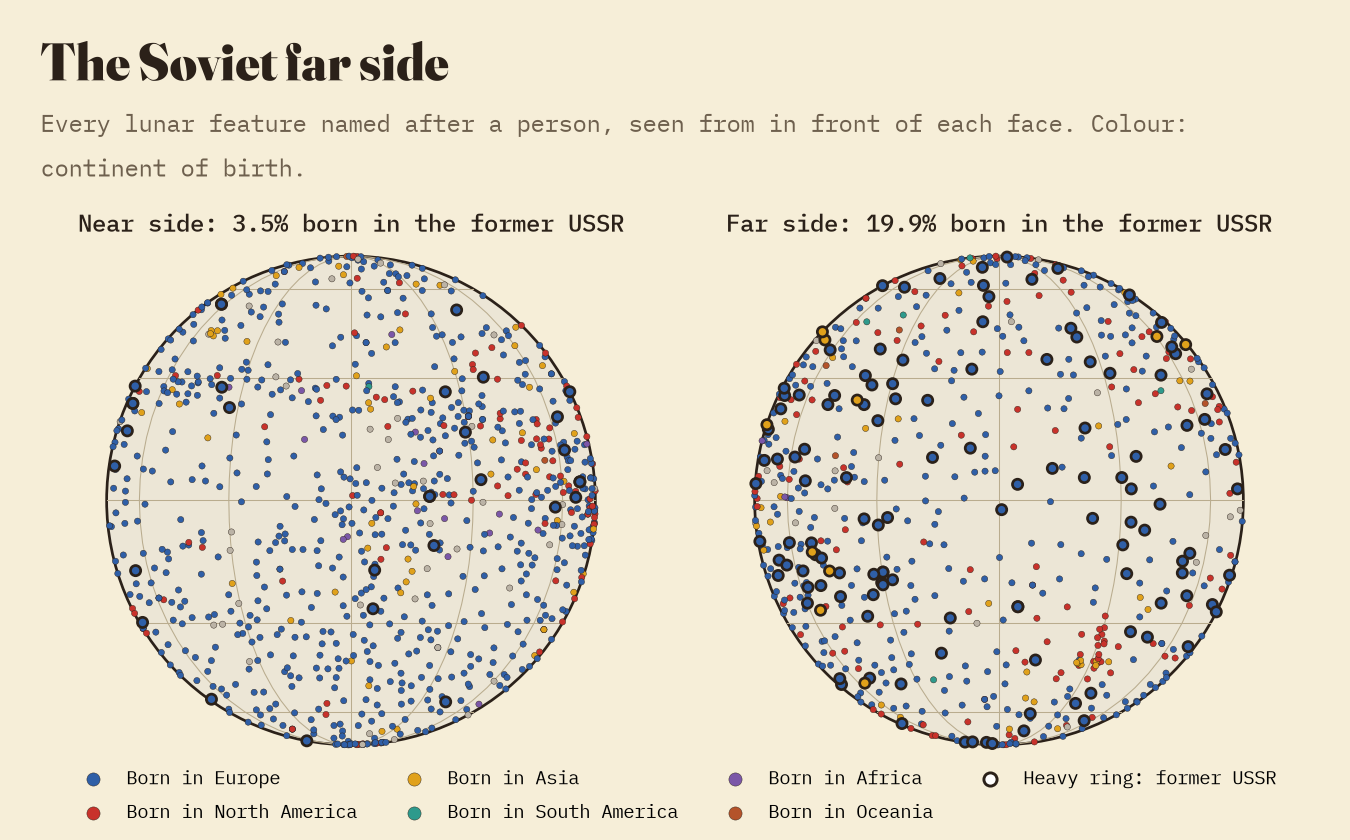
\includegraphics[width=\textwidth]{f_faces.png}
\caption{Lunar features named after people, near side and far side, coloured by continent of birth; heavy rings mark people born in the former Soviet Union.}\label{fig:faces}\end{figure}

\subsection{Birthplaces}
The 1,661 birthplaces are led by the capitals of science: Paris with 69 namings across the four bodies, London 40, Saint Petersburg 37 and Moscow 29 (Table~\ref{tab:towns}, Figure~\ref{fig:towns}). 135 people are honoured on more than one body; Giovanni Schiaparelli, Gerard Kuiper and E. M. Antoniadi on three.

\begin{table}[tbp]\centering\small\caption{The fifteen birthplaces with the most namings.}\label{tab:towns}\begin{tabular}{llrrrrrr}\toprule Birthplace & Country & All & Moon & Mercury & Venus & Mars & People\\\midrule
Paris & France & 69 & 38 & 10 & 16 & 5 & 64\\
London & United Kingdom & 40 & 22 & 3 & 9 & 6 & 36\\
Saint Petersburg & Russia & 37 & 18 & 4 & 13 & 2 & 35\\
Moscow & Russia & 29 & 16 & 4 & 7 & 2 & 28\\
Berlin & Germany & 18 & 13 & 0 & 1 & 4 & 15\\
New York City & United States & 17 & 8 & 3 & 4 & 2 & 16\\
Vienna & Austria & 16 & 12 & 1 & 3 & 0 & 15\\
Boston & United States & 14 & 10 & 3 & 0 & 1 & 13\\
Edinburgh & United Kingdom & 13 & 9 & 1 & 2 & 1 & 11\\
Chicago & United States & 13 & 6 & 1 & 1 & 5 & 11\\
Florence & Italy & 13 & 5 & 4 & 3 & 1 & 13\\
Rome & Italy & 12 & 8 & 1 & 3 & 0 & 11\\
Alexandria & Egypt & 11 & 9 & 0 & 2 & 0 & 10\\
Bologna & Italy & 11 & 8 & 0 & 3 & 0 & 11\\
Odesa & Ukraine & 10 & 8 & 0 & 2 & 0 & 10\\
\bottomrule\end{tabular}\end{table}

\begin{figure}[tbp]\centering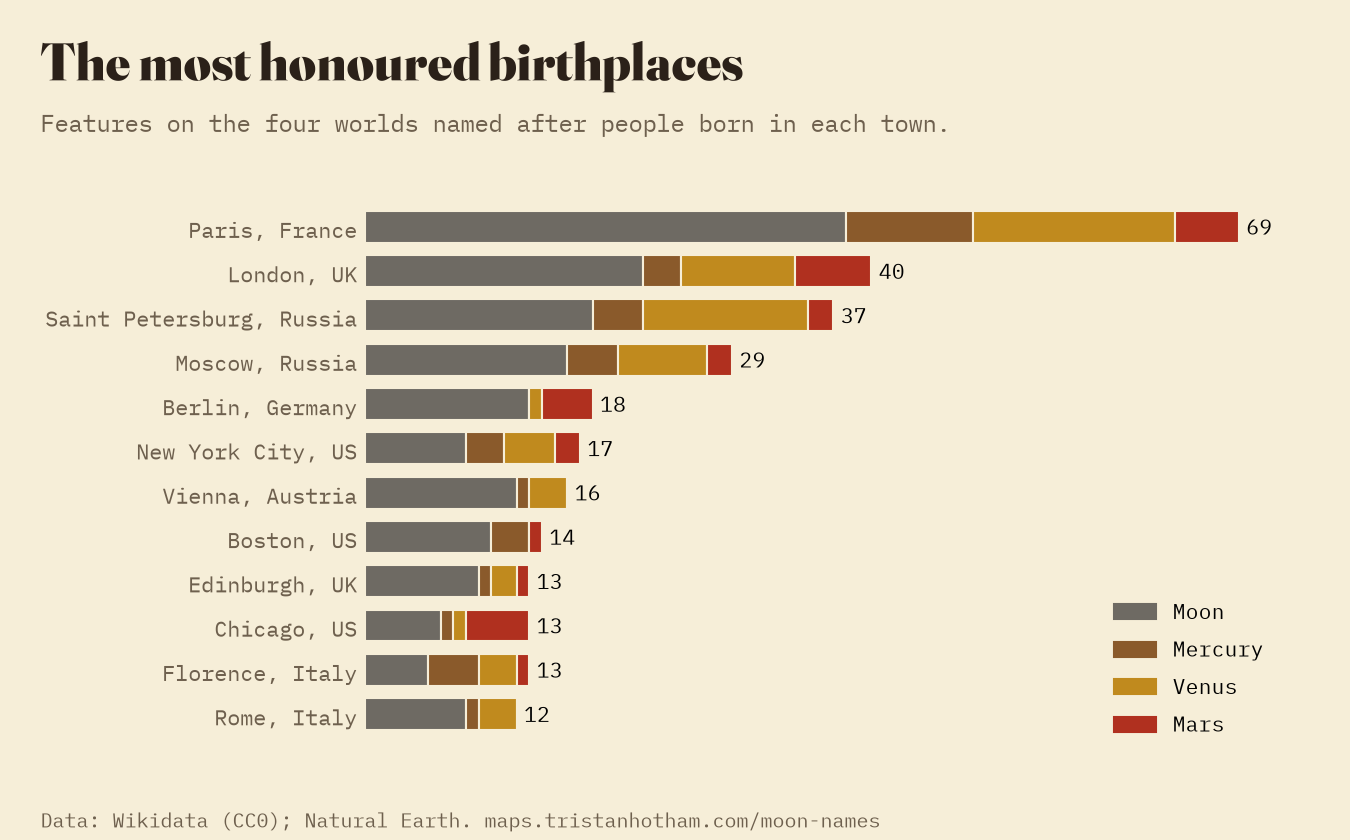
\includegraphics[width=\textwidth]{f_towns.png}
\caption{The twelve birthplaces with the most namings, by body.}\label{fig:towns}\end{figure}

\subsection{Women}
Venus's rule shows in the data: 411 of 412 Venusian namesakes with a recorded sex are women, the exception being Maxwell Montes, named after James Clerk Maxwell before the rule. Elsewhere women are rare (Figure~\ref{fig:women}): 45 of 1,614 lunar namesakes (2.8\%), 17.8\% on Mercury and 5.5\% on Mars, 6.0\% over the three. The share rises with birth date, from 2.6\% of namesakes born before 1800 to 16.7\% of those born from 1900 to 1939 and 30.9\% of the 42 born in 1940 or later. The far side (3.2\%) differs little from the near side (2.5\%).

\begin{figure}[tbp]\centering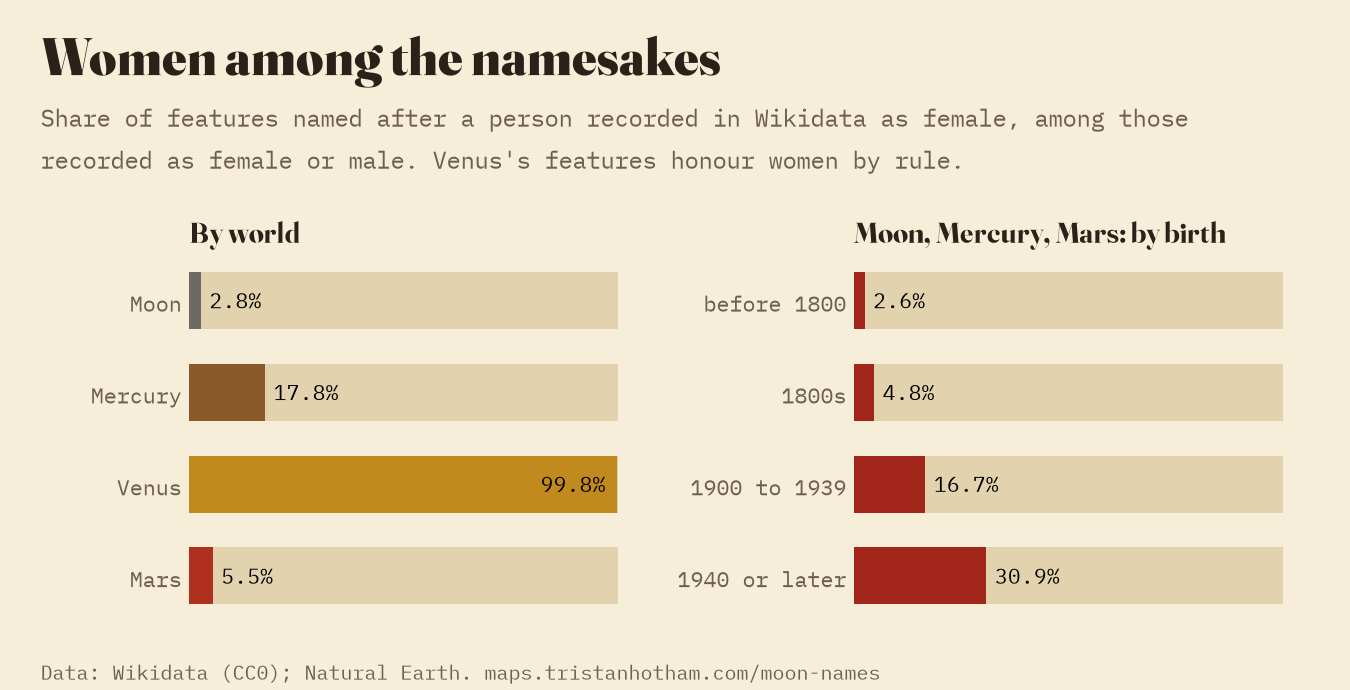
\includegraphics[width=\textwidth]{f_women.png}
\caption{Women among namesakes, by body and by period of birth.}\label{fig:women}\end{figure}

\subsection{The villages of Mars}
Small Martian craters are named after towns and villages of fewer than 100,000 people \citep{gazetteer}. Wikidata gives an Earth namesake with coordinates for 279 Martian features, 217 of them towns and villages, in 102 countries (Figure~\ref{fig:mars}). Their geography is the reverse of Mars's people: 30.4\% are in Europe (against 64.8\% of Mars's namesakes), 29.6\% in Asia and 10.8\% in Africa. The United States (31), India (17) and China (16) have most. On the Moon, 20 features take the names of places on Earth, mostly mountain ranges such as the Alps, Apennines, Carpathians and Caucasus.

\begin{figure}[tbp]\centering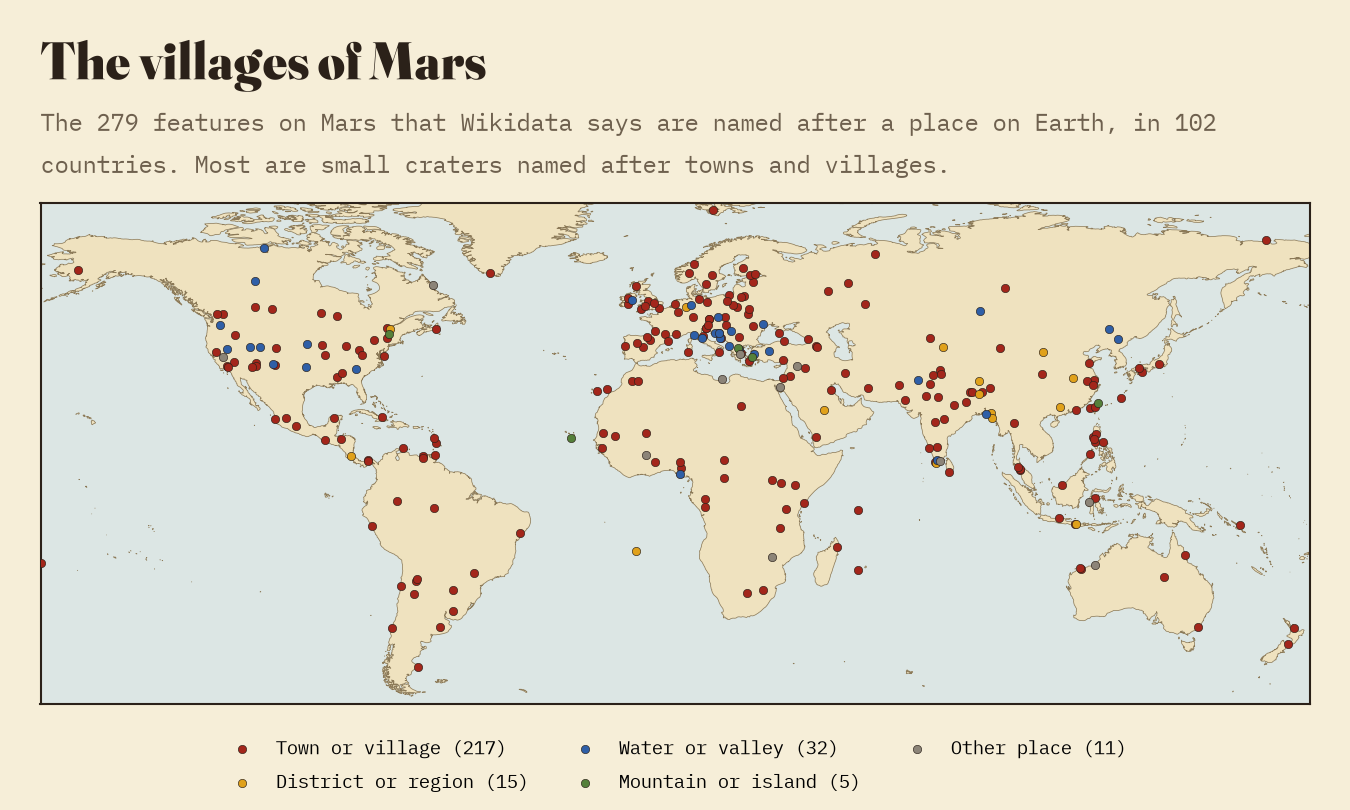
\includegraphics[width=\textwidth]{f_marsplaces.png}
\caption{Places on Earth that features on Mars are named after, by kind.}\label{fig:mars}\end{figure}

\subsection{Errors in the birthplace data}\label{sec:errors}
Wikidata gives Colin Maclaurin (1698 to 1746) a birthplace at a house called The Manse in Victoria, Australia; he was born at Kilmodan, Argyll. I corrected this in a documented overrides file (\texttt{data/overrides\_birthplaces.csv}). I then checked in full every birthplace that Wikidata gives as a country, empire, state or large region, every birthplace whose Wikidata country disagrees with the country it falls in, every missing label and sex value, and all Martian features named after places on Earth. 18 birthplaces are corrected (for example Edna Manley, born in Bournemouth, not Yorkshire, and Gavriil Tikhov, born in Smolevichi, Belarus, not Kazakhstan); 31 people whose Wikidata birthplace is only a country, empire or region, or is disputed, are left unmapped rather than placed at a centroid; 2 contradictory sex values, 3 wrong ``named after'' links, 41 missing labels and 10 place links (ships, a spacecraft, a duplicate item and links to a country or island instead of a town) are corrected. All are listed in the overrides files in \texttt{data/}. To look for similar errors I checked every person born before 1800 with a birthplace in the Americas or Oceania, every pre-1600 birthplace in Africa outside the Mediterranean, and every non-European birthplace that shares its name with a European one (for example Thomas Edison's Milan, Ohio, and Henrietta Swan Leavitt's Lancaster, Massachusetts); all others were plausible. Crimea, which Natural Earth's default view assigns to Russia, is counted as Ukraine.

\section{Limitations}
First, Wikidata is not the IAU Gazetteer. Its coverage of "named after" is good for the Moon and Mercury and weaker elsewhere, and on Mars most features are named after places rather than people (350 of 584, 59.9\%); a second query supplies the coordinates of 279 of them, but some remain unmapped. Second, Wikidata contains errors; I corrected those I could confirm; after the full checks, a fresh random sample of 40 namesakes found 1 with a remaining fault (an unverified ancient birthplace, since removed), but some errors must remain. Third, modern borders assign ancient and imperial birthplaces to today's countries, which is a choice, not a fact about the people. Fourth, occupation groups are coarse and depend on how fully Wikidata lists occupations. Fifth, sex is as Wikidata records it, and the Mars place list is only as complete as Wikidata's "named after" statements.

\section{Conclusion}
The other worlds are named after Europe more than anything else, and the Moon most of all: three in four of its people were born in Europe, and one European city outnumbers three continents. The newer rules for Mercury and Venus have widened the circle, and the Cold War left its mark on the far side. Linking open planetary and biographical data makes these patterns easy to see and to check, and the interactive map lets anyone follow a crater back to a town.

\section*{Data and code availability}
The interactive map is at \url{https://maps.tristanhotham.com/moon-names/}. Data and code are at \url{https://github.com/Tristan-Hotham/moon-names} and archived with this paper at https://doi.org/10.5281/zenodo.24055578. Derived data and text are released under CC BY 4.0 (the Wikidata source is CC0); code under the MIT licence.

\section*{AI statement}
I wrote the text, with drafting and editing assistance from Claude (Anthropic), which also helped prepare the analysis code. I reviewed and checked all text and results.

\begin{thebibliography}{9}
\bibitem[Bast and Buchhold(2017)]{qlever} Bast, H. and Buchhold, B. (2017) QLever: a query engine for efficient SPARQL+Text search. In \textit{Proceedings of the 2017 ACM Conference on Information and Knowledge Management (CIKM)}, 647 to 656.
\bibitem[IAU WGPSN(2026)]{gazetteer} IAU Working Group for Planetary System Nomenclature (2026) Gazetteer of Planetary Nomenclature. USGS Astrogeology Science Center. \url{https://planetarynames.wr.usgs.gov/}
\bibitem[Natural Earth(2026)]{naturalearth} Natural Earth (2026) Admin 0 countries, 1:10m. Public domain. \url{https://www.naturalearthdata.com/}
\bibitem[Riccioli(1651)]{riccioli} Riccioli, G. B. (1651) \textit{Almagestum Novum}. Bologna.
\bibitem[Vrande\v{c}i\'c and Kr\"otzsch(2014)]{wikidata} Vrande\v{c}i\'c, D. and Kr\"otzsch, M. (2014) Wikidata: a free collaborative knowledgebase. \textit{Communications of the ACM} 57(10), 78 to 85.
\bibitem[Whitaker(1999)]{whitaker} Whitaker, E. A. (1999) \textit{Mapping and Naming the Moon: A History of Lunar Cartography and Nomenclature}. Cambridge University Press.
\end{thebibliography}
\end{document}
